%%%%%%%%%%%%%%%%%%%%%%%%%%%%%%%%%%%%%%%%%%%%%%%%%%%%
% LECTURE 25: RADIATION HEAT TRANSFER BETWEEN SURFACES
%%%%%%%%%%%%%%%%%%%%%%%%%%%%%%%%%%%%%%%%%%%%%%%%%%%%
\section*{More on Kirchhoff's law}
\addcontentsline{toc}{section}{More on Kirchhoff's law}

% %%%%%%%%%%%%%%%%%%%%%%%%%%%%%%%%%%%%%%%%%%%%%%%%%%%%
% \subsection*{Exam 2 Review and Course Update}
% \addcontentsline{toc}{subsection}{Exam 2 Review and Course Update}
% %%%%%%%%%%%%%%%%%%%%%%%%%%%%%%%%%%%%%%%%%%%%%%%%%%%%

% \begin{itemize}
%     \item \textbf{Exam 2 statistics:} Highest score = 59 pts, mean = 50.2 pts ($\approx 83.6\%$), standard deviation = 4.8 pts.
%     \item Exam 2 was slightly more challenging than Exam 1 by design; partial credit was awarded generously.
%     \item \textbf{Solutions} will be posted—review these to identify any misunderstandings.
%     \item \textbf{Regrade policy:} You have one week to submit a concise paragraph justifying any requested regrade (no cost to your score).
%     \item \textbf{Final exam preview:}
%     \begin{itemize}
%         \item Worth 30 pts (lower weight than previous exams).
%         \item Format similar to professional-engineer (PC) exam.
%         \item Will include some problems from previous exams.
%         \item One additional lecture on advanced PC-level material will not be exam-eligible.
%         \item A review session will be scheduled.
%     \end{itemize}
% \end{itemize}

% %%%%%%%%%%%%%%%%%%%%%%%%%%%%%%%%%%%%%%%%%%%%%%%%%%%%
% \subsection*{Recap of Radiation Concepts}
% \addcontentsline{toc}{subsection}{Recap of Radiation Concepts}
% %%%%%%%%%%%%%%%%%%%%%%%%%%%%%%%%%%%%%%%%%%%%%%%%%%%%

% In the previous lecture, we introduced numerous concepts related to thermal radiation:

% \begin{itemize}
%     \item \textbf{Directional terminology} based on where light goes and where it comes from:
%     \begin{itemize}
%         \item Emission ($E$): Energy originating from the surface due to its temperature
%         \item Irradiation ($G$): Incoming radiation from external sources landing on a surface
%         \item Reflection ($G_{\mathrm{ref}}$): Portion of irradiation bouncing back from the surface
%         \item Absorption ($G_{\mathrm{abs}}$): Portion of irradiation captured by the material
%         \item Transmission ($G_{\mathrm{tr}}$): Portion of irradiation passing through the material
%         \item Radiosity ($J = G_{\mathrm{ref}} + E$): Total radiation leaving a surface
%     \end{itemize}
    
%     \item \textbf{Surface properties} that characterize radiation interactions:
%     \begin{itemize}
%         \item Reflectivity ($\rho$): Fraction of incident radiation reflected by the surface
%         \item Absorptivity ($\alpha$): Fraction of incident radiation absorbed by the surface
%         \item Emissivity ($\varepsilon$): Ratio of actual emission to black body emission
%         \item Transmissivity ($\tau$): Fraction of incident radiation transmitted through the material
%     \end{itemize}
% \end{itemize}

% A critical distinction: emissivity is solely a property of the surface—if you know the surface and its temperature, you can determine its emissivity. In contrast, absorptivity and reflectivity depend on both the surface properties and the environment (the incoming radiation characteristics).

%%%%%%%%%%%%%%%%%%%%%%%%%%%%%%%%%%%%%%%%%%%%%%%%%%%%
\subsection*{Kirchhoff's Law}
\addcontentsline{toc}{subsection}{Kirchhoff's Law}
%%%%%%%%%%%%%%%%%%%%%%%%%%%%%%%%%%%%%%%%%%%%%%%%%%%%

Due to the complexity of radiation processes, finding useful approximations for quick calculations is valuable. Kirchhoff's Law provides an important simplification.

The complete statement of Kirchhoff's Law is:

\begin{itemize}
    \item For an isothermal enclosure in radiative equilibrium, the total emissivity equals the total absorptivity for all surfaces, regardless of surface properties:
    \[
        \varepsilon_{\mathrm{total}} = \alpha_{\mathrm{total}}
    \]
\end{itemize}

While this is theoretically correct, it applies to thermal equilibrium where no net heat transfer occurs. However, we can apply this law practically when:

\begin{enumerate}[(a)]
    \item $T_{\mathrm{surface}} \approx T_{\mathrm{surrounding}}$ (temperatures are not too far apart)
    \item The radiation environment is large, opaque, and isothermal
\end{enumerate}

Kirchhoff's Law can be extended to more specific cases:
\begin{itemize}
    \item For directional and spectral properties: $\varepsilon_{\lambda,\theta,\phi} = \alpha_{\lambda,\theta,\phi}$
    \item For diffuse surfaces or diffuse radiation: $\varepsilon_{\lambda} = \alpha_{\lambda}$
    \item For gray bodies or black body radiation: $\varepsilon = \alpha$
\end{itemize}

These special cases are particularly useful. If either the radiation is diffuse or the surface is diffuse, we can use $\varepsilon_{\lambda} = \alpha_{\lambda}$. This means either the surface or the environment needs to be diffuse for this relationship to hold.
%
% \begin{table}[h]
% \centering
% \renewcommand{\arraystretch}{1.2} % a touch of vertical padding
% \begin{tabular}{|p{2.8cm}|p{6.2cm}|p{4.0cm}|}
% \hline
% \textbf{Level} & \textbf{Precise statement} & \textbf{Common engineering shorthand} \\ \hline
% \textbf{Spectral} &
% For any surface that is \textbf{in thermodynamic (radiative) equilibrium} with its surroundings at temperature $T$, the \emph{spectral} emissivity equals the \emph{spectral} absorptivity at every wavelength: 
% $\boxed{\varepsilon_{\lambda}(T)=\alpha_{\lambda}(T)}$. &
% “At equilibrium a material emits and absorbs the same fraction of radiation at each wavelength.” \\ \hline
% \textbf{Total / hemispherical} &
% If the surface and its surroundings are at the \textbf{same temperature}, the equality survives the wavelength‑integration, so 
% $\boxed{\varepsilon_{\text{total}}(T)=\alpha_{\text{total}}(T)}$. &
% “When the surface temperature equals the ambient radiation temperature, $\varepsilon=\alpha$.” \\ \hline
% \end{tabular}
% \caption{Kirchhoff’s Law at spectral versus total (hemispherical) levels.}
% \end{table}


% %%%%%%%%%%%%%%%%%%%%%%%%%%%%%%%%%%%%%%%%%%%%%%%%%%%%
% \subsection*{Large, Opaque, Isothermal Enclosure}
% \addcontentsline{toc}{subsection}{Large, Opaque, Isothermal Enclosure}
% %%%%%%%%%%%%%%%%%%%%%%%%%%%%%%%%%%%%%%%%%%%%%%%%%%%%

% For a large, opaque, isothermal enclosure, we can apply a useful simplification:

% \begin{itemize}
%     \item For any point within the enclosure, radiosity equals irradiation: $J = G$
%     \item The black body emission equals both radiosity and irradiation: $E_b = G = J$
%     \[
%         \begin{aligned}
%             &J =\varepsilon E_b+ \rho G
%             \\[0.5em]
%             &J = \textcolor{red}{(1-\rho)} E_b+ \rho G
%             \\[0.5em]
%             &J  = (1-\rho) E_b+\rho G = G
%             \\[0.5em]
%             & (1-\rho) E_b  =(1-\rho) G
%             \\[0.5em]
%             & E_b  =G=J
%         \end{aligned}
%     \]
% \end{itemize}

% This means that regardless of the actual surface properties, we can treat the enclosure as having an effective emissivity of 1 (black body) for calculation purposes. This concept is sometimes called a "black body cavity" or "black cavity" and is used in practical applications and in deriving Kirchhoff's Law.


% \paragraph{Example:} Consider a surface inside a large isothermal enclosure with the following spectral emissivity characteristics:
% \begin{itemize}
%     \item $\varepsilon_{\lambda} = \alpha_{\lambda} = 0.8$ for $\lambda < 3$ $\mu$m
%     \item $\varepsilon_{\lambda} = \alpha_{\lambda} = 0.2$ for $\lambda > 3$ $\mu$m
% \end{itemize}

% \textbf{Part 1:} Calculate the total emissivity as a function of plate temperature.

% To solve this problem, we need to understand where light comes from, what processes it undergoes, and then calculate the total emissivity.

% Total emissivity characterizes what fraction of thermal energy can leave the surface compared to a black body at the same temperature:

% \[
% \varepsilon = \frac{\int_0^{\infty} \varepsilon_{\lambda} E_{b,\lambda} d\lambda}{\int_0^{\infty} E_{b,\lambda} d\lambda}
% \]

% Let's analyze how the Planck distribution shifts with temperature relative to our wavelength threshold of 3 $\mu$m:

% \begin{itemize}
%     \item \textbf{For very low temperatures:} The emission peak occurs at long wavelengths ($\lambda > 3$ $\mu$m). 
    
%     The black body emission curve will have most energy in the region where $\varepsilon_{\lambda} = 0.2$. There will be negligible energy in the shorter wavelengths.
    
%     As the plate temperature approaches absolute zero, about 100\% of emission energy falls in the region where $\varepsilon_{\lambda} = 0.2$, giving a total emissivity of approximately 0.2.
    
%     \item \textbf{For very high temperatures:} The emission peak shifts to short wavelengths ($\lambda < 3$ $\mu$m).
    
%     At extremely high temperatures, approximately 80\% of emission energy falls in the region where $\varepsilon_{\lambda} = 0.8$, with the remaining 20\% at $\varepsilon_{\lambda} = 0.2$, giving a total emissivity approaching 0.8.
    
%     \item \textbf{At intermediate temperatures:} We can use Wien's displacement law to find when $\lambda_{max} = 3$ $\mu$m.
    
%     At $T = 1000$ K, $\lambda_{max} \approx 3$ $\mu$m.
    
%     At this temperature, approximately 25\% of the energy is emitted at wavelengths below 3 $\mu$m (with emissivity 0.8) and 75\% above 3 $\mu$m (with emissivity 0.2).
    
%     The total emissivity is:
%     \[
%     \varepsilon \approx (0.25 \times 0.8) + (0.75 \times 0.2) \approx 0.35
%     \]
% \end{itemize}

% The total emissivity curve would start at 0.2 for low temperatures, pass through approximately 0.35 at 1000 K, and approach 0.8 at very high temperatures.

% \textbf{Part 2:} If the surface is placed inside a large isothermal enclosure with a constant temperature of 300 K, determine the total absorptivity as the plate temperature increases.

% For surroundings at $T_{\infty}=300$ K, the peak wavelength is:
% \[
% \lambda_{max} \approx 10 \text{ } \mu\text{m}
% \]

% This is well into the long wavelength region (> 3 $\mu$m). Almost all of the incident radiation from the 300 K enclosure falls in the spectral region where $\alpha_{\lambda} = 0.2$.

% Therefore, regardless of the plate temperature, the total absorptivity will remain approximately 0.2 as long as the enclosure temperature stays at 300 K.

% This illustrates a key concept: when calculating total emissivity, we use the surface's temperature to determine the spectral distribution. When calculating total absorptivity, we use the surrounding environment's temperature to determine the spectral distribution.

% At the specific condition where $T_{plate} = T_{enclosure} = 300$ K, Kirchhoff's Law ensures that $\varepsilon = \alpha = 0.2$.

%%%%%%%%%%%%%%%%%%%%%%%%%%%%%%%%%%%%%%%%%%%%%%%%%%%%
\subsection*{Gray Surfaces}
\addcontentsline{toc}{subsection}{Gray Surfaces}
%%%%%%%%%%%%%%%%%%%%%%%%%%%%%%%%%%%%%%%%%%%%%%%%%%%%

A gray surface is an approximation where spectral properties (emissivity and absorptivity) are assumed constant across all wavelengths. This creates an apparent circular definition:
\[
    \begin{aligned}
        & \varepsilon_\lambda=\frac{\int_0^{2 \pi} \int_0^{\pi / 2} \varepsilon_{\lambda, \theta} \cos \theta \sin \theta d \theta d \phi}{\int_0^{2 \pi} \int_0^{\pi / 2} 1 \cdot \cos \theta \sin \theta d \theta d \phi}
        \\[1em]
        & \alpha_\lambda=\frac{\int_0^{2 \pi} \int_0^{\pi / 2} \alpha_{\lambda, \theta} I_{\lambda, i} \cos \theta \sin \theta d \theta d \phi}{\int_0^{2 \pi \pi} \int_0^{\pi / 2} I_{\lambda, i} \cos \theta \sin \theta d \theta d \phi}
\end{aligned}
\]
In general, $\varepsilon_\lambda \equiv \alpha_\lambda$. but $\varepsilon_{\lambda, \theta} \equiv \alpha_{\lambda, \theta}$. When
\begin{enumerate}[(i)]
    \item $I_{\lambda, i}$ is NOT a function of ($\theta$, $\phi$) ie., irradiation is diffuse.
    \item $\varepsilon_{\lambda, \theta}$ and $\alpha_{\lambda, \theta}$ are NOT functions of ($\theta, \phi$) i.e., surface is diffuse.
\end{enumerate}
%
We have, $\varepsilon_\lambda=\alpha_\lambda$ for a diffuse surface or diffuse irradiation.

\textbf{}

Similarly, 
\[
    \varepsilon=\frac{\int_0^{\infty} \varepsilon_\lambda E_{\lambda, b}(\lambda, T) d \lambda}{\underbrace{\int_0^{\infty} 1 \cdot E_{\lambda, b}(\lambda, T) d \lambda}_{E_b}}
    \stackrel{?}{=} 
    \frac{\int_0^{\infty} \alpha_\lambda G_\lambda(\lambda) d \lambda}{\underbrace{\int_0^{\infty} 1 \cdot G_\lambda(\lambda) d \lambda}_{G}}=\alpha
\]
%
$\varepsilon=\alpha$ when:
\begin{enumerate}[(i)]
    \item $G_\lambda(\lambda)=c \cdot E_{\lambda, b}(\lambda, T) \longrightarrow G=c \cdot E_b(T)$ irradiation corresponds to emission from a blackbody at the same surface temperature.
    \item The surface is gray ( $\alpha_\lambda$ and $\varepsilon_\lambda$ are independent of $\lambda$ ).
\end{enumerate}
%
we can assume a surface to be gray if.
both surface emission $E_{\lambda, b}$ and irradiation
fall into a region where $\varepsilon_\lambda$ and $\alpha_\lambda$ are approximately constants.
%
\noindent\textbf{View factors for three common three-dimensional geometries}
(the same relations that produce the charts above).

\textbf{Aligned parallel rectangles} $X \times Y$ a distance $L$ apart, with $\bar X = X/L$ and $\bar Y = Y/L$:
\[
F_{ij} = \frac{2}{\pi \bar X \bar Y}\left\{ \ln\!\left[\frac{(1+\bar X^2)(1+\bar Y^2)}{1+\bar X^2+\bar Y^2}\right]^{1/2}
+ \bar X (1+\bar Y^2)^{1/2}\tan^{-1}\!\frac{\bar X}{(1+\bar Y^2)^{1/2}}
+ \bar Y (1+\bar X^2)^{1/2}\tan^{-1}\!\frac{\bar Y}{(1+\bar X^2)^{1/2}}
- \bar X\tan^{-1}\bar X - \bar Y \tan^{-1}\bar Y \right\}
\]

\textbf{Coaxial parallel disks} of radii $r_i$ and $r_j$ a distance $L$ apart, with $R_i = r_i/L$, $R_j = r_j/L$, and $S = 1 + (1+R_j^2)/R_i^2$:
\[
F_{ij} = \tfrac12\left\{ S - \left[S^2 - 4(r_j/r_i)^2\right]^{1/2} \right\}
\]

\textbf{Perpendicular rectangles with a common edge} $X$, the surfaces having widths $Y$ (surface $i$) and $Z$ (surface $j$), with $H = Z/X$ and $W = Y/X$:
\[
F_{ij} = \frac{1}{\pi W}\left( W\tan^{-1}\frac1W + H\tan^{-1}\frac1H - (H^2+W^2)^{1/2}\tan^{-1}\frac{1}{(H^2+W^2)^{1/2}}
+ \frac14 \ln\left\{ \frac{(1+W^2)(1+H^2)}{1+W^2+H^2}\left[\frac{W^2(1+W^2+H^2)}{(1+W^2)(W^2+H^2)}\right]^{W^2}\left[\frac{H^2(1+H^2+W^2)}{(1+H^2)(H^2+W^2)}\right]^{H^2}\right\}\right)
\]


%
\paragraph{Example:} Concentric spheres, find $F_{22}$.
%
\begin{figure}[H]
    \centering
    \begin{tikzpicture}
  % Radii
  \def\rinner{1}
  \def\router{2}
  
  % Draw circles
  \draw[thick] (0,0) circle (\rinner);
  \draw[very thick] (0,0) circle (\router);

  % Points A1 and A2 at angles
  \def\angleA{120}
  \def\angleB{60}
  
  % Coordinates
  \coordinate (A1inner) at (\angleA:\rinner);
  \coordinate (A1outer) at (\angleA:\router);
  \coordinate (A2inner) at (\angleB:\rinner);
  \coordinate (A2outer) at (\angleB:\router);

  % Connectors
  \draw[very thick] (A1inner) -- ++(\angleA:0.2);
  \draw[very thick] (A2outer) -- ++(\angleB:0.8);

  % Dots
  \filldraw (A1inner) circle (2pt);
  \filldraw (A2outer) circle (2pt);

  % Labels
  \node at ($(A1inner) + (\angleA:0.5)$) {\large\textit{$A_1$}};
  \node at ($(A2outer) + (\angleB:1.1)$) {\large\textit{$A_2$}};

\end{tikzpicture}
\end{figure}
%
Using summation Rule: 
\[
    F_{11}+F_{12}=1
\]
Since $A_1$ is convex surface: $F_{11}=0$. Therefore, $F_{12}=1$. Using reciprocity rule: 
\[
    F_{21}=\left(A_1 / A_2\right) F_{12}
\]
Therefore, $F_{21}=\left(A_1 / A_2\right)$
For $A_2$, using summation rule: 
\[
    F_{21}+F_{22}=1
\]
Therefore, $F_{22}=1-\left(A_1 / A_2\right)$
%%%%%%%%%%%%%%%%%%%%%%%%%%%%%%%%%%%%%%%%%%%%%%%%%%%%

\subsubsection*{Fictitious (Hypothetical) Surfaces}
\addcontentsline{toc}{subsubsection}{Fictitious (Hypothetical) Surfaces}
%%%%%%%%%%%%%%%%%%%%%%%%%%%%%%%%%%%%%%%%%%%%%%%%%%%%
When an enclosure contains an opening—such as a door, window, or slot—we often replace that void with a \emph{fictitious} surface to simplify view‑factor bookkeeping.  
Because every ray that leaves a real surface through the opening must eventually impinge on another real surface inside the enclosure (and vice versa), we can relate view factors by

\[
\boxed{%
   F_{\,\text{real} \rightarrow X}
   \;=\;
   \frac{A_{\text{fake}}}{A_{\text{real}}}\;
   F_{\,\text{fake} \rightarrow X}
}
\]

where:
\begin{itemize}
    \item $A_{\text{real}}$ is the area of the actual surface,
    \item $A_{\text{fake}}$ is the area of the fictitious (opening‑cover) surface,
    \item $F_{\text{fake} \rightarrow X}$ is the view factor from the fictitious surface to any other surface $X$ in the enclosure.
\end{itemize}

This construction lets you treat an opening like any other surface, apply the standard reciprocity and summation rules, and then convert the resulting view factors back to the real geometry using the boxed relation.



%%%%%%%%%%%%%%%%%%%%%%%%%%%%%%%%%%%%%%%%%%%%%%%%%%%%
\subsection*{Radiation Exchange between Gray, Diffuse Surfaces}
\addcontentsline{toc}{subsection}{Radiation Exchange between Gray, Diffuse Surfaces}
%%%%%%%%%%%%%%%%%%%%%%%%%%%%%%%%%%%%%%%%%%%%%%%%%%%%
The main difference between gray enclosures and black enclosures is the presence of reflection. In gray enclosures:

\begin{itemize}
    \item Surfaces reflect radiation
    \item Even surfaces that cannot "see" each other directly can exchange energy via reflection
    \item We assume diffuse, gray, opaque surfaces at uniform temperatures
\end{itemize}
%
For practical radiation calculations between surfaces, we make several simplifying assumptions:

\begin{itemize}
    \item Surfaces are diffuse (direction-independent)
    \item Surfaces are gray (wavelength-independent)
    \item Surfaces are opaque (no transmission)
    \item Each surface has uniform temperature
\end{itemize}
%
The radiosity for a gray surface can be expressed as:
\[
J = E + \rho G = \varepsilon E_b + (1-\varepsilon) G
\]

The net energy leaving a surface is:
\[
\frac{q}{A} = J - G = \varepsilon E_b + (1-\varepsilon)G - G = \varepsilon (E_b - G)
\]

This can be rearranged to:
\[
q = \varepsilon A (E_b - G) = \varepsilon A \left(E_b - \frac{J-\varepsilon E_b}{1-\varepsilon}\right) = \frac{\varepsilon A}{1-\varepsilon}(E_b - J)
\]



% The assumption of uniform temperature is particularly important in practice. For surfaces with significant temperature variations, it's better to divide them into smaller elements with approximately uniform temperatures rather than assuming a single temperature for the entire surface.

% \subsubsection*{Switching from Photon Histories to Net Energy Transfer}
% \addcontentsline{toc}{subsubsection}{Switching from Photon Histories to Net Energy Transfer}

% Rather than tracking individual photon paths through multiple reflections (which becomes extremely complex), we focus on the net energy transfer between surfaces. This approach:

% \begin{itemize}
%     \item Ignores the history of each light ray
%     \item Focuses only on whether radiation is leaving a surface (radiosity) or arriving at a surface (irradiation)
%     \item Treats all outgoing radiation the same, whether it's emission or reflection
% \end{itemize}
% \[
%     J=E+\rho G=\varepsilon E_b+\rho G=\varepsilon E_b+(1-\varepsilon) G
% \]
% This simplification works well with diffuse, gray surfaces because:
% \begin{itemize}
%     \item Diffuse surfaces emit and reflect uniformly in all directions
%     \item Gray surfaces treat all wavelengths similarly
%     \item These properties remain constant during multiple reflections
% \end{itemize}

\begin{definition}[Surface Resistance]
\paragraph{Formula}
\begin{figure}[H]
    \centering
    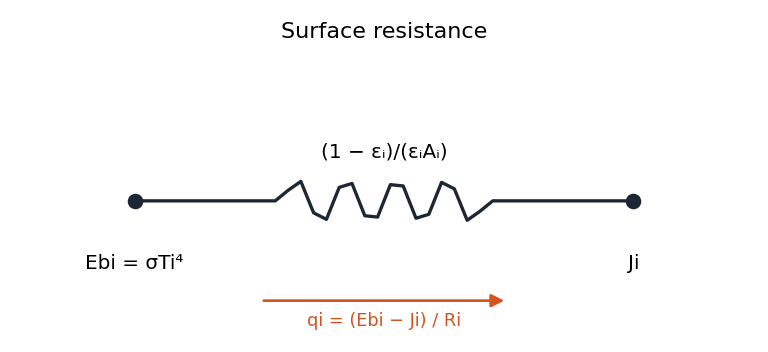
\includegraphics[width=0.6\linewidth]{pics/radiation_network_definiton.png}
\end{figure}
\paragraph{Circuit form}
\textbf{}
\begin{figure}[H]
    \centering
    \begin{circuitikz}
    		% %Grid
    		% \draw[thin, dotted] (0,0) grid (8,8);
    		% \foreach \i in {1,...,8}
    		% {
    		% 	\node at (\i,-2ex) {\i};	
    		% }
    		% \foreach \i in {1,...,8}
    		% {
    		% 	\node at (-2ex,\i) {\i};	
    		% }
    		% \node at (-2ex,-2ex) {0};
    			
    		%Coordinates
    		\coordinate (A) at (3,4);
    		\coordinate (B) at (7,4);
    
    		
    		%Circuit
    		\draw (A) to[resistor, 
                        l^=$(1-\varepsilon_i)/(\varepsilon_i A_i)$, 
                        a_= {}, 
                        v_>, 
                        name=r1, 
                        *-*] (B);
    		
    		%Nodes
    		\node[above left] at (A) {$E_{b,i}$ (surface)};
    		\node[above right] at (B) {$J_i$ (unknown)};
    		
    		% q''
    		\fixedvlen[0.5cm]{r1}{$q_i$}		
    
    \end{circuitikz}
\end{figure}
\end{definition}
%
For each surface $i$ in the enclosure:
\begin{itemize}
    \item Each surface has two nodes:
    \begin{itemize}
        \item An $E_{b,i}$ node representing blackbody emission potential ($E_{b,i} = \sigma T_i^4$)
        \item A $J_i$ node representing radiosity (outgoing radiation)
    \end{itemize}
    \item surface resistance: $R_{s,i} = \frac{1-\varepsilon}{\varepsilon A}$
    \item Heat transfer rate from $E_{b,i}$ to $J_i$: $q_i = \frac{E_{b,i} - J_i}{R_{s,i}}$
\end{itemize}




